\chapter{Números/Relações (4º Bimestre)}

\section{Medidas de tendência central}

In the 4º bimestre of the 5ª série do Ensino Fundamental, we saw how to
construct and interpret various gráficos e tabelas. Given $n$ datos
$x_1, x_2, \ldots, x_n$, we also defined la media (aritmética) de esos
valores as
%%
$$\mu = E(x) =
\overline{x} = \frac{x_1 + x_2 + \ldots + x_n}{n} = \frac{1}{n}\sum_{i=1}^n x_i$$

La moda es el valor lo más repetido en estos datos. Es posible que no sea
única. Si ordenados las valores de menor a mayor, la mediana es el valor de la
variable a la mitad de los datos (si hay un número impar de datos)
o la media de las valores dos variables a la mitad (si hay un número par de
datos).

Now, consideramos datos agrupados en clases
${[a_1, b_1]}, {[a_2, b_2]}, \ldots, {[a_n, b_n]}$ con
$b_1 < a_2, b_2 < a_3 \ldots b_{n-1} < a_n$. Para $1 \leq k \leq n$, la
frecuencia de la clase $[a_k, b_k]$ es $f_k > 0$ y el total es
$N = \sum_{k=1}^n f_k$. La media (aritmética) de estos datos es
%%
$$
\mu = E(x) =
\overline{x} = \frac{1}{N} \sum_{k=1}^n f_k \frac{a_k + b_k}{2}
$$

Para determinar la moda, consideramos el número $k$ tal que la frecuencia $f_k$
es máximal y ponemos
%%
$$
\text{Moda}
= a_k + \left( \frac{f_{k} - f_{k-1}}{{(f_k - f_{k+1})} + {(f_{k} - f_{k-1})}}
\right) \left(b_k - a_k \right)
$$

Aquí, suponemos que $1 < k < n$ y que $f_{k-1}, f_{k+1} < f_k$. Para utilizar
la formula de manera más general, podemos poner $f_0 = f_{n+1} = 0$ y
tomar $M = \frac{a_k+b_k}{2}$ si $f_k = f_{k-1} = f_{k+1}$. Igual al caso
no agrupados, la moda no es definida de manera única si hay muchos
intervalos de frecuencia máximal.

Para definir la mediana, consideramos las frecuencias acumuladas
$F_k = \sum_{i=1}^k f_i$ para $0 \leq k \leq n$ ($F_0 = 0$ y
$F_n = N$). Sea $k$ el menor
entero tal que $F_k \geq \frac{N}{2}$. La mediana es dado por la formula
%%
$$
\text{Mediana} =
a_k + \left( \frac{\frac{N}{2} - F_{k-1}}{f_k}
\right) \left(b_k - a_k \right)
$$

\subsection*{Exercício 1}

Determine las clases, frecuencias y frecuencias acumuladas de estos datos.
Calcule la media, moda y mediana.

\begin{center}
\begin{tabular}{| c | c | c |}
  \hline
  Población (2013) & País o dependencia \\
  \hline
  100 a 200 millones & Brasil, México \\
  \hline
  30 a 100 millones &  Colombia, Argentina, Perú \\
  \hline
  10 a 30 millones & Venezuela, Chile, Ecuador, Guatemala,
  Cuba, Haití, Bolivia \\
  \hline
  1 a 10 millones & República Dominicana, Honduras, Paraguay, El Salvador,
  Nicaragua, Costa Rica, Rico Puerto Rico, Panamá, Uruguay \\
  \hline
  Menos de 1 millión & Guadalupe, Martinica, Guayana Francesa, San Martín,
  San Bartolomé, San Pedro y Miquelón \\
  \hline
\end{tabular}

Fuente: es.wikipedia.org
\end{center}

\subsection*{Exercício 2}

Consideramos datos que podemos agrupar en frecuencias $f_1, \ldots, f_n$:
$x_1 = x_2 = \ldots = x_{F_1} < x_{F_1+1} = x_{F_1+2} = \ldots = x_{F_2} < \ldots
= x_{F_{n-1}} < x_{F_{n-1}+1} = x_{F_{n-1}+2} = \ldots =
x_{F_{n}}$ donde las $F_k$ son las frecuencias acumuladas.
Exprese la media y moda de esos datos no agrupados.

Si consideramos los clases con uno elemento
$a_k = b_k = x_{F_{k-1}} = x_{F_{k-1}+2} = \ldots = x_{F_{k}}$, exprese
la media y moda de esos datos agrupados y compare con las formulas para
datos no agrupados. ¿Que decir de la mediana?

\section{Medidas de dispersão}

Consideramos $n$ datos $x_1, x_2, \ldots, x_n$. Para obtener el rango, restamos
el valor mínimo del valor máximo. La varianza es
%%
$$
V(x) =
\frac{1}{n}
\sum_{i=1}^n \left(x_i - \overline{x}\right)^2
$$
%%
y la desviación típica
%%
$$
\sigma = \sqrt{V(x)}
$$
%%
As an example, consideramos $x_1 = 0, x_2 = 20$ y $x_3 = 10$. La media es
$\frac{0+20+10}{3} = 10$. El rango es $20 - 0 = 20$. La varianza es
$\frac{\left(0-10\right)^2 + \left(10-10\right)^2 + \left(20-10\right)^2}{3}
= \frac{200}{3}$ y la desviación típica
$10 \sqrt{\frac{2}{3}} \approx 8.16$. Si
añadimos los dato $x_4 = 13, x_5 = 17$. La media se vuelve
$\frac{0+20+10+13+17}{5} = 12$. El rango siempre es $20 - 0 = 20$ pero
la varianza es
$\frac{\left(0-12\right)^2 + \left(10-12\right)^2 + \left(20-12\right)^2
+ \left(13-12\right)^2 + \left(17-12\right)^2}{5}
= \frac{238}{5}$ y la desviación típica
$\sqrt{\frac{238}{5}} \approx 6.89$.

Now, consideramos datos agrupados en clases
${[a_1, b_1]}, {[a_2, b_2]}, \ldots, {[a_n, b_n]}$ con
$b_1 < a_2, b_2 < a_3 \ldots b_{n-1} < a_n$. Para $1 \leq k \leq n$, la
frecuencia de la clase $[a_k, b_k]$ es $f_k > 0$ y el total es
$N = \sum_{k=1}^n f_k$.

El rango es $b_n - a_1$. La varianza es
%%
$$
V(x) =
\frac{1}{N}
\sum_{k=1}^n f_k \left(\frac{a_k+b_k}{2} - \overline{x}\right)^2
$$
%%
y la desviación típica queda $\sigma = \sqrt{V(x)}$.

\subsection*{Exercício 3}

Calcule la media, moda y mediana, rango, la varianza y la desviación típica
de estos datos.

\begin{enumerate}
\item $1.60\text{m}, 1.58\text{m}, 1.66\text{m}, 1.72\text{m}, 1.67\text{m}, 1.73\text{m}, 1.65\text{m}, 1.66\text{m}, 1.70\text{m}, 1.80\text{m}$
\item $18 \text{años}, 25 \text{años}, 22 \text{años},  \text{22} \text{años},
   \text{22} \text{años},  \text{18} \text{años},
   \text{24} \text{años},  \text{20} \text{años},  \text{29} \text{años}$
\end{enumerate}

\subsection*{Exercício 4}

Muestre que
%%
$$
V(x) =
\frac{1}{n}
\left(\sum_{i=1}^n x_i^2\right) - \overline{x}^2
$$
%%
\subsection*{Exercício 5}

Calcule el rango, la varianza y la desviación típica de los datos del
Exercício 1.

\section{Amostragem and Normal Distribution}

When observing statistics, it is often important to do some approximations:

\begin{enumerate}
\item The set on which we do observations is called la población estadística.
  Because it is often very large, it is more convenient or even only possible
  to study a small subset, called amostragem estadística.
  We assume that this subset is representativo de la totalidad de la población.
\item We often assume that the statistics in real life follow some abstract
  probabilistic models. For example, when we analyze data obtained from the
  game ``cara'' ou ``coroa'', we assume that the two sides of the coin are
  perfectly symmetric and have the same probability $\frac{1}{2}$ to appear.
  Then we deduce that the game will follow a binomial distribution.
\item Additionally, we assume that the población estadística is large enough to
  tend to the behavior of such probabilistic distribution. Without knowing the
  exact probabilistic distribution, we can show that for a set of data of mean
  $\mu$ and desviación típica $\sigma$, the behavior will tend to the normal
  law ${\mathscr N}(\mu, \sigma^2)$.
  That is, using the notation for datos agrupados en clases, the bar diagram
  $$x \in {[a_i, b_i]} \mapsto f_i$$
  will tend to the function
  $$x \mapsto
  \frac{1}{\sigma \sqrt{2\pi}} e^{-\frac{1}{2} \left(\frac{x-\mu}{\sigma}\right)^2}$$
\end{enumerate}

\subsection*{Exercício 6}

En 2014, la población de Brazil era de 202768562 habitantes.
El número de habitantes inscritos para las elecciones federales eran de
142822046.
A poll Ibope from the 7 to 8 October 2014 was realized on 3010 people
regarding the segundo turno do Eleição presidencial no Brasil and 1324 people
indicated they will vote for Dilma Rousseff

\begin{enumerate}
\item Indique la población estadística correspondiente a la votación y la
  muestra estadística utilizada para estimar el resultado.
\item Determine the percentage of people who indicated they will vote for Dilma
  Rousseff.
\item Dilma Rousseff actually won the election with $51.64\%$ votes. Compare
  with the previous question.
\end{enumerate}

\subsection*{Exercício 7}

We have a bag with three balls $1,2,3$. We pick one random ball, note its
number and put it back into the bag. We perform this operation 100 times and
observe the following results:
3, 3, 3, 3, 3, 1, 1, 2, 3, 3 ;
1, 2, 2, 1, 1, 3, 3, 1, 3, 2 ;
2, 2, 1, 1, 3, 3, 3, 2, 2, 2 ;
3, 2, 3, 2, 1, 1, 3, 2, 3, 1 ;
3, 2, 1, 1, 1, 2, 1, 1, 3, 2 ;
2, 3, 2, 2, 3, 2, 2, 3, 2, 3 ;
3, 3, 1, 1, 1, 3, 2, 2, 2, 1 ;
1, 3, 3, 2, 3, 2, 3, 3, 3, 2 ;
3, 1, 1, 1, 1, 1, 2, 2, 2, 2 ;
2, 1, 2, 1, 2, 1, 3, 1, 1, 2.

\begin{enumerate}
\item Complete the following tables:

\begin{tabular}{| c | c |}
  \hline
  Tries &  Occurences of ball 3 \\
  \hline
  1-10 &   \\
  \hline
  11-20 &  \\
  \hline
  21-30 &  \\
  \hline
  31-40 &  \\
  \hline
  41-50 &  \\
  \hline
  51-60 &  \\
  \hline
  61-70 &  \\
  \hline
  71-80 &  \\
  \hline
  81-90 &  \\
  \hline
  91-100 & \\
  \hline
\end{tabular}

\item
  For each $i=0,1,2,3,4,5,6,7,8,9,10$
  determine the frequence $f_i = \frac{N_i}{10}$
  where $N_i$ is the number of times $i$ appears in the second column.

\item Determine the mean $\mu$ and desviación típica $\sigma$ of the 10 values
  obtained in the previous question.

\item Calculate
  $f(i)=\frac{1}{\sigma \sqrt{2\pi}} e^{-\frac{1}{2} \left(\frac{i-\mu}{\sigma}\right)^2}$
  for $i=0,1,2,3,4,5,6,7,8,9,10$ and compare with the previous results.

\item We start again the experiment and repeat the operation $1000$ times.
  The number of occurences of ball $3$ obtained in the $100$ groups of $10$
  tries is:

  4, 3, 3, 5, 4, 3, 1, 5, 2, 4, 4, 2, 4, 3, 1, 2, 3, 2, 3, 0, 2, 3, 4, 5, 2, 4, 1, 5, 5, 3, 2, 0, 5, 2, 1, 6, 4, 4, 4, 5, 4, 2, 2, 2, 2, 5, 3, 5, 2, 1, 4, 1, 2, 4, 3, 4, 4, 2, 2, 0, 3, 4, 3, 3, 4, 5, 6, 4, 5, 1, 3, 5, 3, 1, 4, 3, 4, 5, 2, 5, 3, 3, 1, 3, 2, 6, 6, 7, 4, 4, 7, 3, 3, 3, 6, 4, 3, 4, 4, 6

  Determine $f_i = \frac{N_i}{100}$, $\mu$, $\sigma$ and $f(i)$.
  Draw a bar diagram $(i,f_i)$ together with the normal function
  $$x \mapsto
  \frac{1}{\sigma \sqrt{2\pi}} e^{-\frac{1}{2} \left(\frac{x-\mu}{\sigma}\right)^2}$$
  for $i=0,1,2,3,4,5,6,7,8,9,10$.
  What do you notice?

\item Interpret the experiment of performing $10$ consecutive tries
  as a binomial law. What are the theorical values of $\mu$ and $\sigma$?
  Compare with the values observed with $10$ and $100$ repetitions of this
  experiment.

\end{enumerate}

\section{Solução do Exercícios}

\subsection*{Exercício 1}

\begin{center}
\begin{tabular}{| c | c | c | c | }
  \hline
  $[a_k, b_k]$ & $f_k$ & $F_k$ \\
  \hline
  $[0,1]$ & $6$ & $6$\\
  \hline
  $[1,10]$ & $9$ & $15$ \\
  \hline
  $[10,30]$ & $7$ & $22$ \\
  \hline
  $[30,100]$ & $3$ & $25$ \\
  \hline
  $[100,200]$ & $2$ & $N=27$ \\
  \hline
\end{tabular}
\end{center}

La media es $\mu = \frac{1}{27} \left(
150 \times 2 + 65 \times 3 + 20 \times 7 + 5.5 \times 9 + 0.5 \times 6 \right)
\approx 25.5 \text{milliones}$. La moda se obtene para el interval $[1,10]$
($f_k=9$):

$$
1 + \frac{9-6}{9-6 + 9-7} \left(10-1\right) = 6.4 \text{milliones}
$$

Tenemos $\frac{27}{2} = 13.5$ entonces la mediana se obtene también para
el interval $[1,10]$. Obtenemos:

$$
1 + \frac{13.5 - 6}{15} \left(10-1\right) = 5.5 \text{milliones}
$$

\subsection{Exercício 2}

La formula de la media es
$\overline{x} =
\frac{1}{N}{\left(x_1 + x_2 + \ldots + x_N\right)} =
\frac{1}{N} {\sum_{k=1}^n \sum_{i=1}^{f_k}  x_{(F_{k-1} + i)}}
$ y entonces
%%
$$
\overline{x} =
\frac{1}{N} {\sum_{k=1}^n f_k a_k}
$$

La moda es el valor $a_k = b_k$ con la frecuencia $f_k$ máximal.

Para datos agrupados, obtenemos $\frac{a_k+b_k}{2} = a_k$ y
$b_k - a_k = 0$. Entonces encuentramos las mismas formulas para la media y la
moda.

De la misma manera, la formula de la mediana para los datos agrupados se vuelve
a $a_{k'}$ para un $1 \leq k' \leq n$. Cuando $N$ es par, es posible que
$F_{k-1} < \frac{N}{2} < F_{k-1}+1$ y la formula de
los datos no grupados es $\frac{b_{k-1}+a_{k}}{2}$ que no coresponde a
un $a_{k'}$. Pero podemos verificar que en otros casos, las formulas son
son equivalentes para datos grupados y no grupados.

\subsection{Exercício 3}

\begin{enumerate}
\item
La media es
$\frac{1.6+1.68+1.66+1.72+1.67+1.73+1.65+1.66+1.7+1.8}{10} = 1.687\text{m}$,
la moda $1.66\text{m}$ (dos veces) y la mediana
$\frac{1.68+1.67}{2} = 1.675\text{m}$.
El rango es $1.80 - 1.58 = 0.22 \text{m} = 22 \text{cm}$.
La varianza es
%%
$$\frac{\left(1.6-1.675\right)^2+\left(1.68-1.675\right)^2+\left(1.66-1.675\right)^2+\left(1.72-1.675\right)^2+\left(1.67-1.675\right)^2+\left(1.73-1.675\right)^2+\left(1.65-1.675\right)^2+\left(1.66-1.675\right)^2+\left(1.7-1.675\right)^2+\left(1.8-1.675\right)^2}{10} =
0.002805$$
%%
 y entonces la desviación típica es
$\sqrt{0.002805} \approx 0.05 \text{m} = 5 \text{cm}$.

\item
La media es $\frac{18+25+22+22+22+24+24+21+20}{9} = 22 \text{años}$.
La moda es $22 \text{años}$ (tres veces) y la mediana es tambíen $22 \text{años}$.
El rango es $25-18 = 7 \text{años}$. La varianza es
$\frac{38}{9} \approx  4.22$ y la desviación típica es
$\sqrt{38}{3} \approx 2 \text{años}$.

\end{enumerate}

\subsection{Exercício 4}

$$
V(x) =
\frac{1}{n}
\sum_{i=1}^n \left(x_i - \overline{x}\right)^2
$$
%%
y $\left(x_i - \overline{x}\right)^2 =
x_i^2 - {2 x_i \overline{x}} + \overline{x}^2$ entonces
%%
$$
V(x) =
\frac{1}{n}
\left(\sum_{i=1}^n x_i^2\right)
- \frac{2}{n}
\left(\sum_{i=1}^n x_i\right) \overline{x}
+ \frac{n}{n} \overline{x}^2
$$
%%
y finalmente $V(x) =
\frac{1}{n}
\left(\sum_{i=1}^n x_i^2\right) - 2\overline{x}^2 + \overline{x}^2 =
\frac{1}{n}
\left(\sum_{i=1}^n x_i^2\right) - \overline{x}^2$.

\subsection{Exercício 5}

El rango es $200 - 0 = 200 \text{milliones}$. La varianza es
%%
$$
V =
\frac{1}{27}
\left(
2 \times \left(150 - \mu \right)^2 +
3 \times \left(65 - \mu \right)^2 +
7 \times \left(20 - \mu \right)^2 +
9 \times \left(5.5 - \mu \right)^2 +
6 \times \left(0.5 - \mu \right)^2
\right) \approx 1602
$$
%%
y la desviación típica $\sigma = \sqrt{V} \approx 40 \text{milliones}$.

\subsection*{Exercício 6}

\begin{enumerate}
\item La población estadística correspondiente a la votación es el conjunto de
  los habitantes inscritos para las elecciones federales. La muestra
  estadística es el conjunto de los 3010 personas que fueron interrogadas.
\item $\frac{1324}{3010} = 44\%$
\item Besides the fact that people may not have made their final choice or
  may not want to tell it, the sample is not perfectly representative of
  the whole population.
\end{enumerate}

\subsection*{Exercício 7}

\begin{enumerate}
\item We find

\begin{tabular}{| c | c |}
  \hline
  Tries &  Occurences of ball 3 \\
  \hline
  1-10 &  7 \\
  \hline
  11-20 & 3 \\
  \hline
  21-30 & 3 \\
  \hline
  31-40 & 4 \\
  \hline
  41-50 & 2 \\
  \hline
  51-60 & 4 \\
  \hline
  61-70 & 3 \\
  \hline
  71-80 & 6 \\
  \hline
  81-90 & 1 \\
  \hline
  91-100 & 1 \\
  \hline
\end{tabular}

\item We find
$f_0=0$,
$f_1=0.2$,
$f_2=0.1$,
$f_3=0.3$,
$f_4=0.2$,
$f_5=0$,
$f_6=f_7=0.1$ and
$f_8=f_9=f_{10}=0$

\item $\mu=3.4$ and $\sigma \approx 1.85472$.

\item We find
$f(0)\approx0.0400788$,
$f(1)\approx0.0931184$,
$f(2)\approx0.161774$,
$f(3)\approx0.210151$,
$f(4)\approx0.20413$,
$f(5)\approx0.148263$,
$f(6)\approx0.0805214$,
$f(7)\approx0.0326995$,
$f(8)\approx0.0099294$,
$f(9)\approx0.00225453$,
$f(10)\approx0.000382773$.
  These are relatively different from the values of $f_i$.

\item We now find
$f_0=0.03$,
$f_1=0.09$,
$f_2=0.18$,
$f_3=0.23$,
$f_4=0.25$,
$f_5=0.14$,
$f_6=0.06$,
$f_7=0.02$ and
  $f_8=f_9=f_{10}=0$ ;
  $\mu=3.34$ and $\sigma \approx 1.53766$ ;
$f(0)\approx0.0245197$,
$f(1)\approx0.0815021$,
$f(2)\approx0.177477$,
$f(3)\approx0.253182$,
$f(4)\approx0.236616$,
$f(5)\approx0.144869$,
$f(6)\approx0.0581064$,
$f(7)\approx0.0152684$,
$f(8)\approx0.00262834$,
$f(9)\approx0.000296408$,
  $f(10)\approx0.000021898$.
  We notice that increasing the number of observation makes the approximation
  of the $f_i$ (blue) with a normal law $x \mapsto f(x)$ (orange) more accurate:

  \begin{center}
    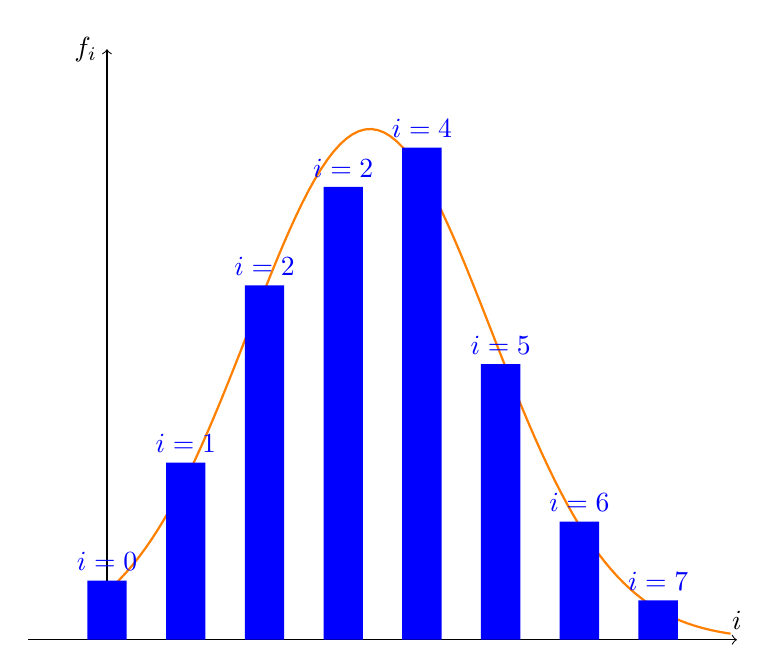
\begin{tikzpicture}[yscale=.25]
    \draw[->] (-1,0) -- (8,0) node[above] {$i$};
    \draw[->] (0,0) -- (0,30) node[left] {$f_i$};
    \draw[orange,thick] (0,2.4519701726788625)--(0.08,2.741617758793015)--(0.16,3.057194498575924)--(0.24,3.399880693696482)--(0.32,3.7707585841571896)--(0.4,4.1707890296805665)--(0.48,4.600787343034513)--(0.56,5.061398595205235)--(0.64,5.553072757186636)--(0.72,6.076040084487414)--(0.8,6.630287186838795)--(0.88,7.2155342555886035)--(0.96,7.8312139435003)--(1.04,8.476452404832376)--(1.12,9.150053006480851)--(1.2,9.850483212634124)--(1.28,10.575865125052145)--(1.36,11.323970128250174)--(1.44,12.092218043360084)--(1.52,12.877681136419282)--(1.6,13.677093256820195)--(1.68,14.486864300536936)--(1.76,15.303100101797941)--(1.84,16.12162775772034)--(1.92,16.93802628502548)--(2,17.747662398569073)--(2.08,18.545731090544727)--(2.16,19.32730057953588)--(2.24,20.087361092890063)--(2.32,20.820876846993013)--(2.4,21.522840500697185)--(2.48,22.188329280039518)--(2.56,22.812561909871654)--(2.64,23.390955442218893)--(2.72,23.919181043799405)--(2.8,24.393217797440048)--(2.88,24.80940358489044)--(2.96,25.164482151993937)--(3.04,25.455645510997474)--(3.12,25.680570908082455)--(3.2,25.83745167554079)--(3.28,25.92502139545269)--(3.36,25.94257092283113)--(3.44,25.88995794816861)--(3.52,25.767608919022493)--(3.6,25.576513284346017)--(3.68,25.31821017022323)--(3.76,24.99476773798246)--(3.84,24.60875561190636)--(3.92,24.163210890670108)--(4,23.661598371237755)--(4.08,23.107765713608526)--(4.16,22.505894357338487)--(4.24,21.86044706447041)--(4.32,21.17611300722124)--(4.4,20.4577513418929)--(4.48,19.710334212944286)--(4.56,18.938890113493542)--(4.64,18.148448491736147)--(4.72,17.343986438364965)--(4.8,16.530378219979475)--(4.88,15.71234833993348)--(4.96,14.894428713621457)--(5.04,14.080920442553577)--(5.12,13.275860563524077)--(5.2,12.48299403855487)--(5.28,11.705751140840487)--(5.36,10.947230284230836)--(5.44,10.210186241249023)--(5.52,9.497023599366095)--(5.6,8.80979521904104)--(5.68,8.15020538133252)--(5.76,7.5196172487801585)--(5.84,6.919064211446083)--(5.92,6.349264650839852)--(6,5.8106396279081425)--(6.08,5.303332987014495)--(6.16,4.827233365232148)--(6.24,4.3819976044413265)--(6.32,3.967075081573485)--(6.4,3.5817324986324097)--(6.48,3.2250787074916722)--(6.56,2.8960891835040825)--(6.64,2.5936298052308544)--(6.72,2.316479643702422)--(6.8,2.0633525122180663)--(6.88,1.8329170755331357)--(6.96,1.623815364244828)--(7.04,1.4346795852854548)--(7.12,1.2641471618330133)--(7.2,1.1108739749792553)--(7.28,0.9735458146427401)--(7.36,0.8508880781228918)--(7.44,0.7416737811537393)--(7.52,0.6447299682630278)--(7.6,0.5589426267263108)--(7.68,0.48326022158549437)--(7.76,0.4166959783242294)--(7.84,0.3583290451766585)--(7.92,0.3073046690614452);

    \fill[blue] (-.25,0) -- (-.25,3) --
    (0,3) node[above]{$i=0$} -- (.25,3) -- (.25,0) -- cycle;

    \fill[blue] (.75,0) -- (.75,9) --
    (1,9) node[above]{$i=1$} -- (1.25,9) -- (1.25,0) -- cycle;

    \fill[blue] (1.75,0) -- (1.75,18) --
    (2,18) node[above]{$i=2$} -- (2.25,18) -- (2.25,0) -- cycle;

    \fill[blue] (2.75,0) -- (2.75,23) --
    (3,23) node[above]{$i=2$} -- (3.25,23) -- (3.25,0) -- cycle;

    \fill[blue] (3.75,0) -- (3.75,25) --
    (4,25) node[above]{$i=4$} -- (4.25,25) -- (4.25,0) -- cycle;

    \fill[blue] (4.75,0) -- (4.75,14) --
    (5,14) node[above]{$i=5$} -- (5.25,14) -- (5.25,0) -- cycle;

    \fill[blue] (5.75,0) -- (5.75,6) --
    (6,6) node[above]{$i=6$} -- (6.25,6) -- (6.25,0) -- cycle;

    \fill[blue] (6.75,0) -- (6.75,2) --
    (7,2) node[above]{$i=7$} -- (7.25,2) -- (7.25,0) -- cycle;

\end{tikzpicture}
\end{center}

\item It is a binonimal law with parameter $n=10$ tries and
  $p=\frac{1}{3}$ (probability of picking ball $3$ at each step).
  We have $\mu = np = \frac{10}{3} \approx 3.333$ and
  $\sigma = \sqrt{n p {(1-p)}} \approx 1.4907$.
  The experiment repeated 10 times gave $\mu=3.4$ and $\sigma \approx 1.85472$
  while the experiment repeated 100 times gave
  $\mu=3.34$ and $\sigma \approx 1.53766$. Again, we see that by using
  more measures we obtained a better approximation.
\end{enumerate}
